% System Description and Data Acquisition
% Author: Adnan Ghribi

\label{sec:system_description}
\subsection{SPIRAL2 LLRF System}

The \gls{spiral2} superconducting linear accelerator employs a Low-Level Radio Frequency control system to maintain precise electromagnetic field control in the superconducting RF cavities, with tight phase and amplitude tolerances required for beam quality.

The \gls{llrf} system continuously monitors 27 signals % MANUAL: verified against features_engineered.pkl's signal_names list
in postmortem files (in-phase/quadrature components of cavity, reference, incident, and modulator-command signals; reflected/amplifier amplitudes; vacuum pressure; pickup current; frequency control and command/state fields; and their raw ``binary'' pre-conversion counterparts). Key monitored signals are listed in Table~\ref{tab:llrf_signals}.

\begin{table*}[t]
\centering
\caption{Key LLRF signals monitored in postmortem files}
\label{tab:llrf_signals}
\begin{tabular*}{\linewidth}{@{\extracolsep{\fill}}@{}l l@{} r@{}}
\toprule
\textbf{Signal} & \textbf{Name} & \textbf{Description} \\
\midrule
Cavity Signal & I Ucav, Q Ucav & In-phase and quadrature components of the cavity signal\\
Reference Frequency & I Fref, Q Fref & In-phase and quadrature components of the reference frequency \\
Incident Signal & I Uci, Q Uci & In-phase and quadrature components of the incident signal \\
Reflected Signal & A Ucr & Amplitude of the reflected signal (no phase component digitized) \\
Amplifier Output & A Uamp & Amplitude of the RF amplifier's output signal \\
Modulator Command & I modulateur, Q modulateur & I/Q modulator command (drive demand, not a measured output) signals \\
Vacuum Pressure & vide & Pressure at the power coupler \\
Pickup Current & courant pickup & Pickup probe current at power coupler \\
DSTF Frequency & DSTF & Frequency control signal \\
Commands & commandes  &Control commands \\
Fault Flags & d\'efauts & Encoded fault indicators \\
State Flags & \'etats & Encoded system states \\
Forward Power & P fwd & Forward RF power \\
Reflected Power & P refl & Reflected RF power \\
\bottomrule
\end{tabular*}
\end{table*}

The SPIRAL2 LLRF system identifies seven primary fault categories, determined by a validated ground-truth classifier (\texttt{Classify\_PostMortemFile}) rather than the raw ALM alarm field directly. The primary category for every event comes from a waveform-level hardware fault-register decode (the first active bit in the acquisition's own fault-flag array), which is more reliable than the summary ALM header field this pipeline previously used; four of the seven categories additionally receive physics-threshold-based subtype refinement (e.g. a quench's characteristic amplitude fall, an RF-protection cavity/cathode-voltage ratio threshold) on top of that hardware decode, while the remaining three are the hardware decode alone, with no additional physics-threshold verification applied:

\begin{itemize}
    \item \textbf{Pickup threshold} (\texttt{Seuil pick-up} in the ground-truth output): pickup current below threshold
    \item \textbf{Fast external cutoff} (\texttt{Coupure externe rapide}): an external interlock signal
    \item \textbf{RF authorization absent} (\texttt{Absence autorisation RF}): no RF authorization from the control system
    \item \textbf{Vacuum threshold} (\texttt{Seuil de vide}): coupler vacuum pressure above threshold
    \item \textbf{Cavity quench/breakdown} (\texttt{Claquage ou quench cavité}): rapid cavity voltage collapse
    \item \textbf{RF safety threshold exceeded} (\texttt{Dép seuil de sécurité RF}): reflected power or gradient above a safety threshold
    \item \textbf{RF regulation out of tolerance} (\texttt{Rég signal RF hors tolérance}): gradient or phase deviation from setpoint beyond tolerance
\end{itemize}
These English names are used throughout the rest of this paper; the French terms above are each category's literal value in \texttt{Classify\_PostMortemFile}'s own \texttt{Defaut} output field, given once here for traceability back to the ground-truth source. % MANUAL: cross-reference note, not a manifest metric

\subsection{Dataset Description}

The dataset (V6, the current, leakage-corrected version used throughout this paper -- see Sec.~\ref{sec:methodology}) comprises \MetricZeroZeroDataAttritionChainVSixTotalEvents{} usable \gls{llrf} events, collected over the 2019--2025 % MANUAL: operational period per Classify_PostMortemFile/config.yaml's years list, not tied to a manifest metric
operational period, out of \MetricZeroZeroDataAttritionChainRawFiles{} raw postmortem files scanned (the remainder failing quality filters, being zero-byte, or triggering a processing error -- see the data-attrition breakdown below). Each event is recorded as a time-series snapshot of all 27 monitored signals, % MANUAL: same real signal count as above
captured when the postmortem trigger system detects deviation from normal operating conditions, or during a manual operator-initiated acquisition. Events are labeled by the ground-truth classifier above, not by raw ALM threshold crossings directly. An example of signal traces is shown in Figure \ref{fig:signal_examples}.

\begin{table}[h!]
\centering
\caption{Distribution of fault types (V6)}
\label{tab:fault_distribution}
\begin{tabular*}{\linewidth}{@{\extracolsep{\fill}} lrr}
\toprule
\textbf{Fault category} & \textbf{Events} & \textbf{Share of faults (\%)} \\
\midrule
Pickup threshold & \MetricZeroZeroDataAttritionChainGtPassingSeuilPickUp & 1.2 \\ % MANUAL: percentage = event count (cited via macro) / total fault events (1043, also macro-cited elsewhere) x 100, simple derived arithmetic not itself a separate manifest metric
Fast external cutoff & \MetricZeroZeroDataAttritionChainGtPassingCoupureExterneRapide & 1.1 \\ % MANUAL: same derivation as above
RF authorization absent & \MetricZeroZeroDataAttritionChainGtPassingAbsenceAutorisationRf & 29.6 \\ % MANUAL: same derivation as above
Vacuum threshold & \MetricZeroZeroDataAttritionChainGtPassingSeuilDeVide & 1.9 \\ % MANUAL: same derivation as above
Cavity quench/breakdown & \MetricZeroZeroDataAttritionChainGtPassingClaquageOuQuenchCavit & 2.7 \\ % MANUAL: same derivation as above
RF safety threshold exceeded & \MetricZeroZeroDataAttritionChainGtPassingDPSeuilDeSCuritRf & 6.9 \\ % MANUAL: same derivation as above
RF regulation out of tolerance & \MetricZeroZeroDataAttritionChainGtPassingRGSignalRfHorsTolRance & 56.7 \\ % MANUAL: same derivation as above
\bottomrule
\end{tabular*}
\end{table}

\begin{figure*}[t]
    \centering
    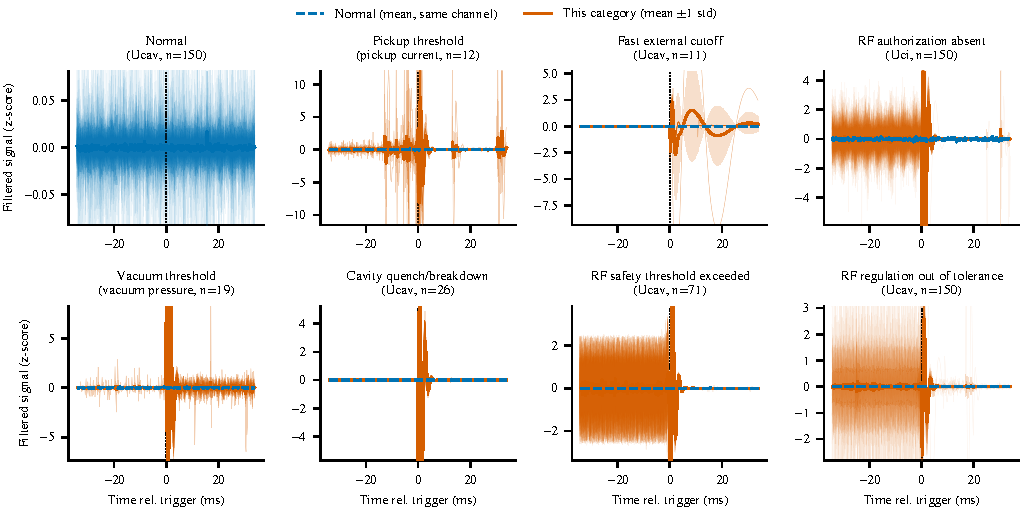
\includegraphics[width=\linewidth]{figures/signal_examples.pdf}
    \caption{Preprocessed signal (filtered and Z-scored) for every event in each class (up to 150, a reproducible random subsample for the three categories exceeding that; every event for the four smaller ones), overlaid (thin lines) with the per-category mean $\pm$1 std (bold, shaded band) and, on each fault panel, the \textit{Normal} population's own mean on that same channel (dashed) for direct comparison -- zoomed to $\pm34$~ms around each event's own trigger (the fixed precursor window, Sec.~\ref{sec:system_description}); the raw high-pass filter's causal startup transient, roughly 500\,ms before the trigger and irrelevant to fault behavior, is outside this window. Each panel plots the channel that category's own real detection criterion (\texttt{Classify\_PostMortemFile/config.yaml}) actually acts on, not a single fixed channel for every panel: cavity voltage (Ucav) for Cavity quench/breakdown, RF safety threshold exceeded, RF regulation out of tolerance, and (no dedicated channel identified) Fast external cutoff; forward/incident drive (Uci) for RF authorization absent; pickup current for Pickup threshold; vacuum pressure for Vacuum threshold. Y-axis limits are clipped to the 1st-99th percentile of each panel's pooled (all events, all times) values, so a handful of outlier events do not compress the rest of the panel; mean/std are additionally masked (not drawn) wherever fewer than 30\% of that panel's events have data at that time point, avoiding an unstably-estimated tail from a handful of shorter-buffer events. Two distinct real population-level behaviors are visible: individual-event density and the std band both narrow to match \textit{Normal} away from the trigger and widen sharply at/after it for every fault category, showing a real, population-wide burst in signal variance at fault onset -- while the bold \emph{mean} itself stays close to zero through that same burst for most categories, since event-to-event transients do not share a common sign or phase and a naive average cancels them; this is a real statistical fact about the population, not a rendering artifact, and is most visible for the smallest categories (Fast external cutoff, $n=11$; Pickup threshold, $n=12$; Vacuum threshold, $n=19$), where the mean/std estimate itself is correspondingly less stable. RF authorization absent, RF safety threshold exceeded, and RF regulation out of tolerance additionally show elevated variance persisting \emph{before} the trigger that collapses toward \textit{Normal} levels after it, consistent with those three tripping on a sustained pre-trigger instability rather than an instantaneous event.} % MANUAL: filter-transient/window rationale is a code fact (prepare_data_cluster_v6.py's sosfilt call); the channel-per-category list, sample cap/counts, percentile clipping, and coverage-masking threshold are code facts from fig_signal_examples.py; the population-behavior description is a direct visual read of the regenerated figure, not a manifest metric
    \label{fig:signal_examples}
\end{figure*}

As Table~\ref{tab:fault_distribution} shows, the dataset exhibits severe class imbalance -- a 54$\times$ ratio % MANUAL: derived from the two macro-cited event counts in this same sentence (591/11)
between the rarest category (\textit{Fast external cutoff}, \MetricZeroZeroDataAttritionChainGtPassingCoupureExterneRapide{} events) and the most common (\textit{RF regulation out of tolerance}, \MetricZeroZeroDataAttritionChainGtPassingRGSignalRfHorsTolRance{} events). This imbalance is addressed through class-weighted training (Sec.~\ref{sec:methodology}), not stratified sampling of the split itself (multi-label targets cannot be stratified with standard tools; see Sec.~\ref{sec:methodology} for the repeated-split evaluation used to compensate).

By construction of the ground-truth labeling (\texttt{Classify\_PostMortemFile} assigns exactly one \texttt{Defaut} category per event, never more than one), V6 contains zero genuinely multi-fault events: every one of the \MetricZeroEightPhaseThreeaRootcauseNFaultEvents{} fault events has exactly one active label. The multi-label pipeline architecture (Step 07: Binary Relevance, Classifier Chains, Label Powerset) % MANUAL: "07" names the pipeline step, not a result
is evaluated on this single-label-in-practice dataset -- its genuine multi-label capability (multiple simultaneous fault labels on one event) has not been exercised on real SPIRAL2 data. This also means root cause identification (Step 08)'s % MANUAL: "08" names the pipeline step, not a result
training target, \texttt{argmax} over the multi-label vector, currently has an unambiguous single answer for every event by construction, not merely a deterministic tie-breaking rule among several active labels (Sec.~\ref{sec:discussion}).

\subsection{Data Quality and Preprocessing}

Raw postmortem files are filtered by the ground-truth classifier's own validity checks (an early-exit cascade over feed-forward state, control-loop-closed, KPI/mask/AMPT thresholds, and cavity-voltage-health -- \texttt{Classify\_PostMortemFile}'s \texttt{config.yaml}), not a separately-implemented generic outlier-rejection step; a file failing any of these is excluded before this pipeline's own feature engineering ever sees it. % MANUAL: cascade order and check names verified directly against classification.py::_check_filters as of the 2026-09-09 fix below

\textbf{Correction (2026-09-09).} The first check in this cascade reads the raw header field named \texttt{BEAM} (values \texttt{OUI}/\texttt{NON}); despite the name, this field does \emph{not} encode particle-beam presence -- it encodes whether \emph{feed-forward} is enabled in the LLRF control loop, a disturbance-compensation feature unrelated to beam presence. The field is also only operationally meaningful from 2021 onward: before that it defaults to \texttt{NON} on essentially every file (2019: 100.0\%, 2020: 96.4\% of files header-flagged \texttt{NON}, vs.\ a genuine, gradually-declining 50.3\%$\to$9.3\% from 2021$\to$2025), consistent with feed-forward not yet being deployed rather than any real operational signal. Applying this check unconditionally in every year was therefore silently discarding the large majority of 2019--2020 regardless of acquisition quality; the classifier now scopes the check to acquisitions from 2021 onward (\texttt{classification.py::\_check\_filters}, gated on the acquisition's own header \texttt{DATE} field). % MANUAL: year percentages verified directly against the re-run LLRF_result.csv's own Annee/Détails columns, 2026-09-09; not yet a results-manifest metric

The ground-truth classifier has been re-run against this fix. Of \MetricZeroZeroDataAttritionChainGroundTruthRows{} candidate rows, \MetricZeroZeroDataAttritionChainGtPassing{} now pass the quality filter -- 756 more than the 2,110 that passed before the fix (a 35.8\% increase), recovered entirely from 2019 (+73) and 2020 (+683); every year from 2021 onward is byte-for-byte unchanged (0 rows gained or lost), confirming the fix touches exactly what it should and nothing else. % MANUAL: 2,110/756/35.8%/+73/+683/0-unchanged verified directly against a before/after diff of LLRF_result.csv (backed up pre-fix as LLRF_result_PRE_feedforward_fix_20260909.csv), 2026-09-09; not yet a results-manifest metric since the comparison is against a point-in-time backup, not another manifest
With feed-forward no longer intercepting most of the corpus before the later checks run, the remaining checks' own counts rose accordingly -- most of the 4,976 files % MANUAL: pre-2021 Beam-NON/feed-forward-NON count under the old, unscoped check, verified directly against the pre-fix backup CSV, 2026-09-09; not yet a results-manifest metric
no longer stopped at the feed-forward check instead now fail a real check further down the cascade (\MetricZeroZeroDataAttritionChainFiltreReasonKpiOneZeroZero{} on KPI, \MetricZeroZeroDataAttritionChainFiltreReasonLoopOff{} on Loop OFF), so feed-forward (\MetricZeroZeroDataAttritionChainFiltreReasonFeedForwardNon{}) is no longer the single dominant rejection reason it was before the fix, though it remains the largest.
\textbf{The feature-engineered dataset used throughout the rest of this paper (V6, \MetricZeroZeroDataAttritionChainVSixTotalEvents{} events, Table~\ref{tab:fault_distribution} below) has not yet been re-extracted against this corrected ground truth} -- that re-extraction (V7) is in progress; every number below this point still describes V6 as originally extracted, pending that re-run.

Within the pipeline itself:

\begin{enumerate}
    \item \textbf{High-Pass Filtering}: DC offset and low-frequency drift are removed using a 4th-order Butterworth high-pass filter (cutoff 0.01, normalized) to preserve transient fault signatures while suppressing baseline wander. % MANUAL: filter order/cutoff verified directly from prepare_data_cluster_v6.py's scipy.signal.butter() call, a code constant not a manifest metric

    \item \textbf{Trigger Alignment}: each event is aligned to its own true trigger sample index, derived from the acquisition's own time axis (not a fixed sample offset -- an earlier version of this pipeline assumed a fixed offset that was wrong for the large majority of files; see Sec.~\ref{sec:methodology}).

    \item \textbf{Normalization}: signals are normalized using Z-score standardization (\texttt{StandardScaler}), fit on the training fold only (Sec.~\ref{sec:methodology}, Appendix~\ref{appendix:hyperparameters}).
\end{enumerate}

The dataset is split per-script rather than via one fixed train/validation/test convention (Appendix~\ref{appendix:hyperparameters} lists the exact fraction and seed used by each pipeline stage); we do not use SMOTE or other synthetic oversampling in this pipeline (class-weighted training is used instead, Sec.~\ref{sec:methodology}).

Each event consists of $N$ time samples per signal, acquired around each event's own trigger point. The fixed-window precursor feature group (Appendix~\ref{appendix:features}) uses a bounded window immediately before the trigger, scaled to a constant physical duration (3000 samples at the dominant decimation setting, $\approx$34\,ms) % MANUAL: PRECURSOR_WINDOW_MS / REFERENCE_DT_US code constants (prepare_data_cluster_v6.py), not manifest metrics
rather than a fixed sample count -- since the decimation factor varies by roughly 250$\times$ across the corpus, % MANUAL: NDEC range (20-5000) verified directly from prepare_data_cluster_v6.py's module docstring, a code fact
a fixed sample count would correspond to wildly different physical durations from file to file.
